\documentclass[tikz,border=6pt]{standalone}
\usepackage{tikz}
\usepackage{amsmath,bm}
\usetikzlibrary{shapes.geometric, shapes.arrows, arrows.meta, positioning,
                fit, backgrounds, calc, decorations.pathreplacing}

\definecolor{markovblue}{RGB}{31,119,180}
\definecolor{renewgreen}{RGB}{44,160,44}
\definecolor{stateorange}{RGB}{230,136,28}
\definecolor{decisionyellow}{RGB}{240,210,60}

\begin{document}
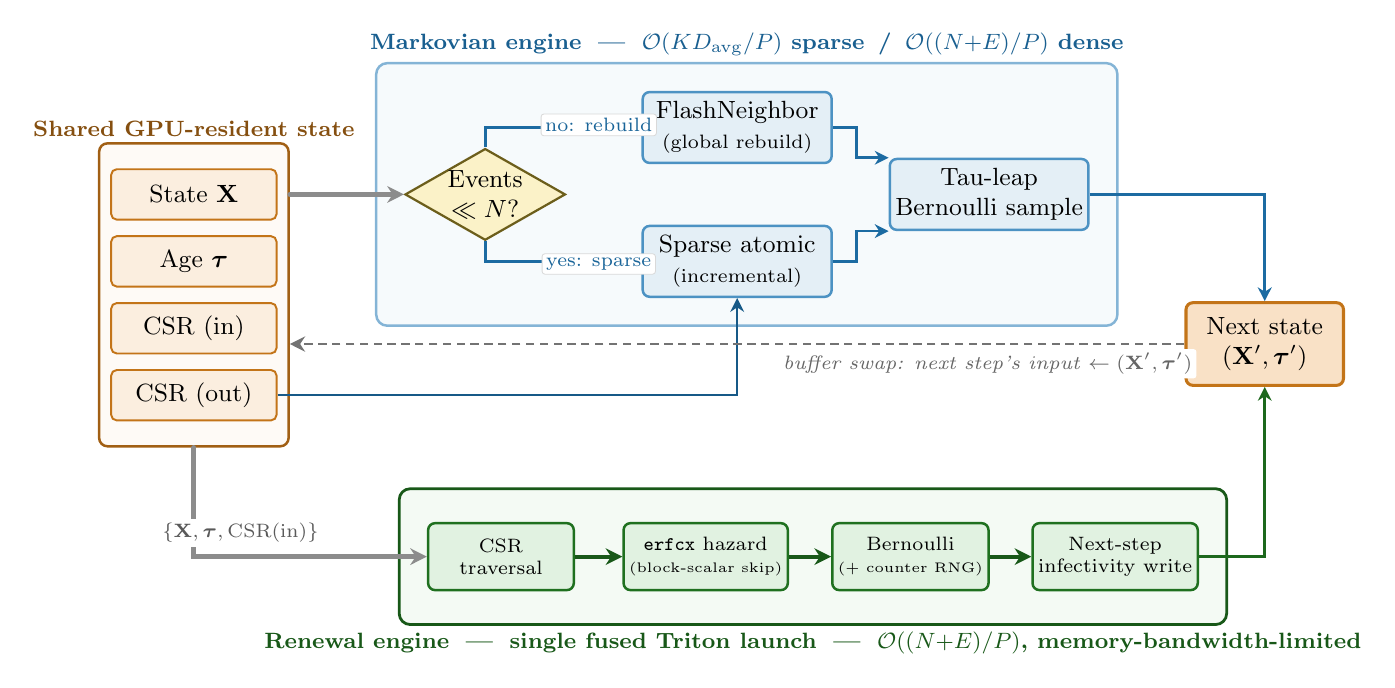
\begin{tikzpicture}[
    % ---------------- node styles ----------------
    state/.style={rectangle, draw=stateorange!85!black, line width=0.7pt,
                  rounded corners=2pt, fill=stateorange!14,
                  minimum width=2.1cm, minimum height=0.64cm,
                  align=center, font=\small, inner sep=2pt},
    mkernel/.style={rectangle, draw=markovblue!80, line width=0.9pt,
                    rounded corners=2.5pt, fill=markovblue!12,
                    minimum width=2.4cm, minimum height=0.9cm,
                    align=center, font=\small, inner sep=2pt},
    rkernel/.style={rectangle, draw=renewgreen!70!black, line width=0.9pt,
                    rounded corners=2.5pt, fill=renewgreen!14,
                    minimum width=1.85cm, minimum height=0.85cm,
                    align=center, font=\scriptsize, inner sep=2pt},
    decision/.style={diamond, draw=decisionyellow!45!black, line width=0.8pt,
                     aspect=1.75, inner sep=0pt, align=center,
                     font=\small, fill=decisionyellow!28},
    outstate/.style={rectangle, draw=stateorange!85!black, line width=1.1pt,
                     rounded corners=2.5pt, fill=stateorange!25,
                     minimum width=2cm, minimum height=1.05cm,
                     align=center, font=\small, inner sep=2pt},
    % ---------------- arrow styles ----------------
    mflow/.style={-{Stealth[length=5pt,width=5pt]}, line width=1pt,
                  color=markovblue!90!black},
    rflow/.style={-{Stealth[length=5pt,width=5pt]}, line width=1pt,
                  color=renewgreen!65!black},
    pipe/.style={-{Stealth[length=6pt,width=6pt]}, line width=1.4pt,
                 color=renewgreen!55!black},
    bundle/.style={-{Stealth[length=6pt,width=6pt]}, line width=1.8pt,
                   color=black!45, line cap=round},
    feedback/.style={-{Stealth[length=5.5pt,width=5.5pt]}, line width=1pt,
                     color=black!55, densely dashed},
    % ---------------- label styles ----------------
    elabel/.style={font=\footnotesize\bfseries, inner sep=2pt},
    branchlabel/.style={font=\scriptsize, inner sep=1.5pt,
                        fill=white, rounded corners=1pt,
                        draw=black!15, line width=0.3pt},
    buslabel/.style={font=\scriptsize\itshape, fill=white, inner sep=1.5pt,
                     rounded corners=1pt, text=black!65}
]

%======================================================================
% (1) SHARED STATE COLUMN
%======================================================================
\node[state] (Xs)     at (0, 2.25) {State $\mathbf{X}$};
\node[state] (tau)    at (0, 1.40) {Age $\bm{\tau}$};
\node[state] (csrin)  at (0, 0.55) {CSR (in)};
\node[state] (csrout) at (0,-0.30) {CSR (out)};

\begin{scope}[on background layer]
    \node[fit=(Xs)(tau)(csrin)(csrout),
          draw=stateorange!70!black, line width=0.9pt,
          fill=stateorange!4, rounded corners=3pt,
          inner xsep=4pt, inner ysep=9pt,
          label={[elabel, text=stateorange!58!black]
                 above:Shared GPU-resident state}] (gpustate) {};
\end{scope}

%======================================================================
% (2) MARKOVIAN ENGINE
%======================================================================
\node[decision] (mode)   at (3.7,  2.25) {Events\\$\ll N$?};
\node[mkernel]  (flashN) at (6.9,  3.10) {FlashNeighbor\\\scriptsize{(global rebuild)}};
\node[mkernel]  (sparse) at (6.9,  1.40) {Sparse atomic\\\scriptsize{(incremental)}};
\node[mkernel]  (taulp)  at (10.1, 2.25) {Tau-leap\\Bernoulli sample};

% State X -> decision (bundled data flow)
\draw[bundle] (gpustate.east|-mode) -- (mode.west);

% decision branches: path + label placed with text= (not color=)
\draw[mflow] (mode.north) |- (flashN.west);
\node[branchlabel, text=markovblue!85!black]
      at ($(mode.north)!0.5!(flashN.west) + (0.45, 0.16)$) {no: rebuild};

\draw[mflow] (mode.south) |- (sparse.west);
\node[branchlabel, text=markovblue!85!black]
      at ($(mode.south)!0.5!(sparse.west) + (0.45,-0.16)$) {yes: sparse};

% branches converge on tau-leap
\draw[mflow] (flashN.east) -- ++(0.3,0) |- (taulp.north west);
\draw[mflow] (sparse.east) -- ++(0.3,0) |- (taulp.south west);

\begin{scope}[on background layer]
    \node[fit=(mode)(flashN)(sparse)(taulp),
          draw=markovblue!55, line width=0.9pt,
          fill=markovblue!4, rounded corners=4pt,
          inner xsep=10pt, inner ysep=10pt,
          label={[elabel, text=markovblue!80!black]
                 above:Markovian engine
                       \;\textemdash\; $\mathcal{O}(K D_{\mathrm{avg}}/P)$
                       sparse \,/\, $\mathcal{O}((N{+}E)/P)$ dense}]
          (markovbox) {};
\end{scope}

%======================================================================
% (3) RENEWAL ENGINE -- pipelined fused kernel
%======================================================================
\node[rkernel] (r1) at (3.9,  -2.35) {CSR\\traversal};
\node[rkernel] (r2) at (6.5,  -2.35) {\texttt{erfcx} hazard\\\tiny(block-scalar skip)};
\node[rkernel] (r3) at (9.1,  -2.35) {Bernoulli\\\tiny(+ counter RNG)};
\node[rkernel] (r4) at (11.7, -2.35) {Next-step\\infectivity write};

% pipeline arrows
\draw[pipe] (r1.east) -- (r2.west);
\draw[pipe] (r2.east) -- (r3.west);
\draw[pipe] (r3.east) -- (r4.west);

% Bundled state -> renewal engine: drop straight down from the shared
% state column and then bend horizontally at the renewal engine's row,
% so the arrow enters r1 at the same level as the Renewal Engine.
\draw[bundle]
     (gpustate.south) |- (r1.west) coordinate[pos=0.6] (bundleMid);
\node[buslabel] at ($(bundleMid)+(0,0.30)$)
     {$\{\mathbf{X},\bm{\tau},\mathrm{CSR}(\mathrm{in})\}$};

% CSR(out) -> Sparse atomic: go RIGHT under sparse, then UP into sparse.south
\draw[mflow, line width=0.9pt, color=markovblue!75!black]
     (csrout.east) -| (sparse.south);

\begin{scope}[on background layer]
    \node[fit=(r1)(r2)(r3)(r4),
          draw=renewgreen!55!black, line width=1pt,
          fill=renewgreen!5, rounded corners=4pt,
          inner xsep=10pt, inner ysep=12pt,
          label={[elabel, text=renewgreen!55!black]
                 below:Renewal engine \;\textemdash\;
                        single fused Triton launch \;\textemdash\;
                        $\mathcal{O}((N{+}E)/P)$, memory-bandwidth-limited}]
          (renewbox) {};
\end{scope}

%======================================================================
% (4) OUTPUT
%======================================================================
\node[outstate] (out) at (13.6, 0.35)
      {Next state\\$(\mathbf{X}',\bm{\tau}')$};

\draw[mflow] (taulp.east) -| (out.north);
\draw[rflow] (r4.east) -| (out.south);

%======================================================================
% (5) FEEDBACK LOOP -- straight horizontal line through the middle
%     corridor between Markov (y>=0.64) and Renewal (y<=-1.51) containers
%======================================================================
\coordinate (fbEnd) at (gpustate.east |- out.west);

\draw[feedback] (out.west) -- (fbEnd);

\node[font=\scriptsize\itshape, color=black!60, inner sep=1.5pt,
      fill=white, rounded corners=1pt]
     at ($(out.west)!0.22!(fbEnd)+(0,-0.25)$)
     {buffer swap: next step's input $\leftarrow (\mathbf{X}',\bm{\tau}')$};

\end{tikzpicture}
\end{document}